\documentclass[main.tex]{subfiles}

\begin{document}

\section{Offer Networks}
An \textbf{offer network} instance can be formally modeled as a directed graph where vertices $t \in T$ represent tasks and labeled directed edges $(t_a,t_b) : u_1$ represent an offer by user $u_1$ to do task $t_a$ in exchange requested task $t_b$.
\begin{center}
  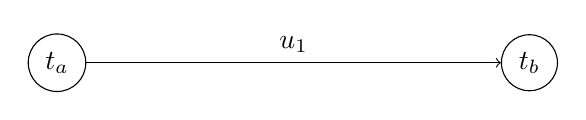
\begin{tikzpicture}
    \node[draw, circle] (ta) at (0,0) {$t_a$};
    \node[draw, circle] (tb) at (6,0) {$t_b$};
    \path [->] (ta) edge node[above] {$u_1$} (tb);
  \end{tikzpicture}
\end{center}

A matching of users who can satisfy each other is a vertex cycle. See the simplest case below:

\begin{center}
  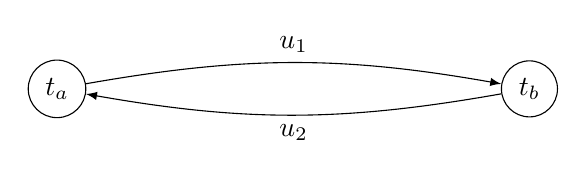
\begin{tikzpicture}
    \node[draw, circle] (ta) at (0,0) {$t_a$};
    \node[draw, circle] (tb) at (6,0) {$t_b$};
    \draw[-latex] (ta) to[bend left=10] node[above] {$u_1$} (tb);
    \draw[-latex] (tb) to[bend left=10] node[below] {$u_2$ }(ta);
  \end{tikzpicture}
\end{center}


\end{document}
